\documentclass[runningheads]{llncs}
\usepackage{graphicx}
\usepackage{graphicx}
\usepackage{bm}
\usepackage{amsmath}
\usepackage{amssymb}
\usepackage{booktabs}
\usepackage{threeparttable}
\usepackage[ruled]{algorithm2e}
\usepackage{setspace}
\usepackage{float}
\usepackage{caption}
\usepackage{array}
\usepackage{url}
\usepackage{subfigure}

%\newcommand{\figref}[1]{Fig.\ref{#1}}
%\newcommand{\eqnref}[1]{Eq.\ref{#1}}
%\newcommand{\tref}[1]{Table.\ref{#1}}

\title{A Serverless Solution for Fair Exchange System \\
	\large{Report of CSC8109 Group Project}} % Title
\author{Christopher Clark \and Tong Zhou \and Weicheng Yang \and Junyan Wang}
\institute{School of Computing, Newcastle University \\ Newcastle upon Tyne, NE4 5TG}

\begin{document}
\maketitle


%=============================
%=== Introduction ============
%=============================
\section{Introduction} 


%=============================
%=== System Specification ====
%=============================
\section{System Specification} 
According to the requirements described in CSC8109 Group Project Specification, this project is aimed to design and develop a fair exchange system on the AWS cloud. The general process is defined as the following picture\cite{csc8109}:

	\begin{figure}[H]
		\centering
		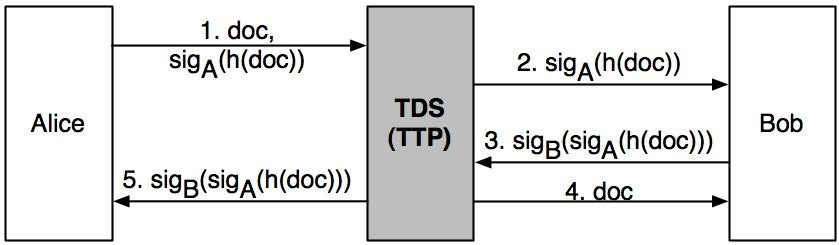
\includegraphics[width=10cm]{reportpics/1.jpg}  
		\caption{Process}
		\label{Process}
	\end{figure}

Before we start to discuss the design of the system, firstly we define some words that will generally be used within our system to represent the components in the fair exchange system:

\begin{itemize}
	\item \textbf{User:} any party who use our system to conduct any fair exchange processes;
	\item \textbf{Sender:} the user who initiates a new exchange request to send some document to another party;
	\item \textbf{Receiver:} the user who passively receive an exchange request from another party;
	\item \textbf{TDS (Trusted Document Store):} a third-party server that works as a fair operator that make sure no party during the exchange can have an advantage over the others, also called a Trusted Third Party(TTP);
	\item \textbf{EOO (Evidence Of Original):} the signature of the document encrypted by the private key of the sender. This signature can be used as evidence of the original document that is confirmed and signed by the sender;
	\item \textbf{EOR (Evidence Of Receipt):} the signature if the EOO that encrypted by the private key of the receiver. This signature can be used as evidence that the receiver has already got the target document;
	\item \textbf{Transaction:} an entire life cycle from when sender send the document with EOO to system till receiver got the document with validated EOO and, at the same time, sender got the validated EOR from the receiver. Any exchange aborted during any point of the exchange can also be regarded as a transaction;
\end{itemize}

As is shown in the given diagram, there are three parties involved within this system, which is a sender(Alice), a receiver(Bob) and TDS. The sender is trying to send a document to the receiver, at the same time exchange the EOO with EOR. The TDS works as a fair third party which makes sure that no party can have an advantage over the other one, in another word, either receiver get the document with the EOO and at the same time sender get the EOR, or none of them get anything from the other party. 

\subsection{Workflow}
To be specific, there are five steps in the entire workflow.

\begin{enumerate}
	\item The sender sends the document and EOO to TDS.
	\item TDS send the signature to Receiver.
	\item The receiver sends the EOR to TDS.
	\item TDS send the document to Receiver.
	\item TDS send the EOR to Sender.
\end{enumerate}

But, as a trusted third party, several validation steps that not listed in the diagram should also be included within the process:

\begin{itemize}
	\item Between step 1 and step 2, TDS need to validate whether the EOO match with the document, so that sender cannot cheat by sending a fake EOO that does not match with the document;
	\item Between step 3 and step 4, TDS need to validate whether EOR matches with the EOO that stored in TDS, so that sender cannot cheat by sending a fake EOR that is not generated by the given EOO.
\end{itemize}

Moreover, both the sender and receiver should be available to abort the transaction manually if they want to terminate the process. But according to fair exchange principles, there are several restricts that should be applied to the manually abort process, which is that neither sender or receiver can abort a transaction after receiver got the document. Also, they cannot abort a transaction that has not been created.

\subsection{Key Generation}
During the exchange process, the system frequently needs to generate some signature as proof that some user has confirmed of some specific operation. Thus, we will need some secured key for every user in our system before any transaction been conducted. We can ask the user to provide their private key every time before the transaction, but that will be easier if we assign a pre-generated private key for every user when a new user is registered in our system.

\subsection{Authentication}
To distinguish the sender and receiver from all users, we need to have some user authentication mechanisms that only allow identified user to use our system, and also we need to have the registration process before a new user start to use our system. The registration process should include the following procedures:

\begin{itemize}
	\item Get user information include:
		\begin{itemize}
			\item Email
			\item Full name
			\item Password (may be kept by third-party authentication service)
		\end{itemize}
	\item Verify the email by sending a verification code to the email address.
	\item Generate a private key and a public key so that it can be used as the unique signa-ture of a particular user.
\end{itemize}

After the user has been created in our system, the user can log in to our systemwith the email address and password set by this user.

\subsection{Exchange process}
To provide service to the user with all kind of devices and platform, we are goingto design a browser-based system that allows users from all over the world to accessour system and communicate with TDS server.


%=============================
%=== Background Research ====
%=============================
\section{Background Research} 
The background research is going to be broken down into 3 main sub-sections. It will talk at a high level at a high level about the architectural styles that are offered by AWS. This is turn will reflect on the language that we have chosen, which will logically follow on how the Cryptography Libraries/Technologies that were used.
\begin{itemize}
	\item Technology Alternatives/Choices Within AWS
	\item Cryptography Libraries
\end{itemize}

\subsection{Technology Alternatives/Choices within AWS}
This was the first major hurdle that we had to consider when designing our system. This section is not going to talk about the specific AWS services that were used within he making of this project, more so; the choice that is seen as the most viable will influence the type of technologies within AWS that we intend to utilize. 

There are two routes that can be taken when looking at the subject of architecture. It can be looked at from the perspective of how the code base isgoing to be structured. Is it a valid option to go for a monolithic code base, ora fine grained microservices based architecture when it comes to structuring the codebase. However, upon looking into the two main types of architecturethat are popular with current cloud services, it was seen that this decision is somewhat made for you.

In reference to the decision being made for you in terms of how you architectyour overall cloud service. This is in reference to an extremely popular cloud architecture known as Serverless.

\subsection{What is Serverless?}
Serverless is a somewhat new concept within Cloud Computing. This is not necessarily the concept of not using servers. More so, it is the concept of not having to manage your own servers, and having an only pay for what you use mentality. The main benefits of serverless are as follow:
\begin{enumerate}
	\item No Server Management
	\item Flexible Scaling
	\item Pay for Value
	\item Automated High Availability
\end{enumerate}

With Serverless it isn't necessarily all or nothing either. AWS offers Serverlesscomponents such as databases, web servers, and code bases. To get a betteridea of what this means in all 3 contexts. A serverless database would only be running when it is being used; so if it is being written and read from, you will only pay when it is active. When it is lying dormant, you are not paying for that time. In contrast to having a standard server set up with a; database,application container (Jboss / tomcat) and web server; which may be running 24/7 without being used.

In reference to Serverless not having to be all or nothing, there may be use cases where a serverless database and application container(something to run your code) is fine. However, you may need to control access to who can access you website (such as it only being accessible from Newcastle University). This is something that is not offered by Serverless, and will be mentioned in the later sections; so using an EC2 server may be the way to go.

Other drawbacks of not utilizing a serverless architecture can include If you want an EC2 instance running then you need to pay someone to apply software patches, check the disk space, make sure there is enough CPU  etc. This costs money - which you don't need if you are using a serverless architecture. Also if you go from 2 users of your platform to 1,000,000 then you will need to scale your EC2 instances which can be pain.  They will required load balancers and autoscaling groups.

\subsection{Cryptography Libraries}
Our cryptography research can be split up into 3 main sections.
\begin{itemize}
	\item What kind of keys did we choose
	\item What kind of verification algorithm did we use
\end{itemize}
There are more elements to be discussed in terms of cryptography, in terms of how did we handle key storage and generation? But this is more appropriately discussed in section 3. So within the spec, it was suggested to look at the following components of the JCA library :
\begin{itemize}
	\item KeyStore for representation of a (file-based) certificate and key store (for management of certificates and public/private key pairs). You can use the Java command line keytool utility to generate a keystore, keys and associated certificates.
	\item Signature for generation and verification of signatures over data.
	\item SignedObject for encapsulation of a signature and its associated object(data).
	\item Cipher for encryption and decryption of data.
	\item MessageDigest for generation and verification of secure hashes of data.
	\item SecureRandom for generation of secure pseudo random numbers.
\end{itemize} 
At the point of deciding on how to implement our encryption, the group had agreed that they would feel comfortable doing a lot of the implementation in Javascript. Firstly because of the front end implementation being done in this language, but also the fact that using Serverless technologies such as Lambda lend themselves very well to using this Language. 

So the challenge at this point then became, finding something that implements the above within JavaScript, and do we need all of these featuresing the first place?

Through looking at various node packages, we found various keys within the npm store, however there was not a lot of official verification on these, so wedidn't feel these would necessarily be safe.

In the end we ended up using the official Cryptography library offered by Node. This allowed us to generate keys (RSA/DSA) that could be used for the generation of signed Objects backed by the X-509 standard, similar to the JCA libraries. We opted to use the RSA keys, as they verify much faster than DSA keys. And the speed at which DSA keys can create a signature is not that much faster than an RSA key.

In terms of actual encryption of our data, it was assumed we would be using secured means of communication backed by HTTPS/SSL mentioned in the spec, as well as using a storage repository that offers encryption at rest such as S3; the encryption of our data wouldn't be necessary.

%=============================
%=== Design Decisions ====
%=============================
\section{Design Decisions}
This section is going to deal with the selection of specific selection of AWS Services. What they are, and why they were chosen. How they were applied to the algorithm is going to be discussed in section 5.

	\begin{figure}[H]
		\centering
		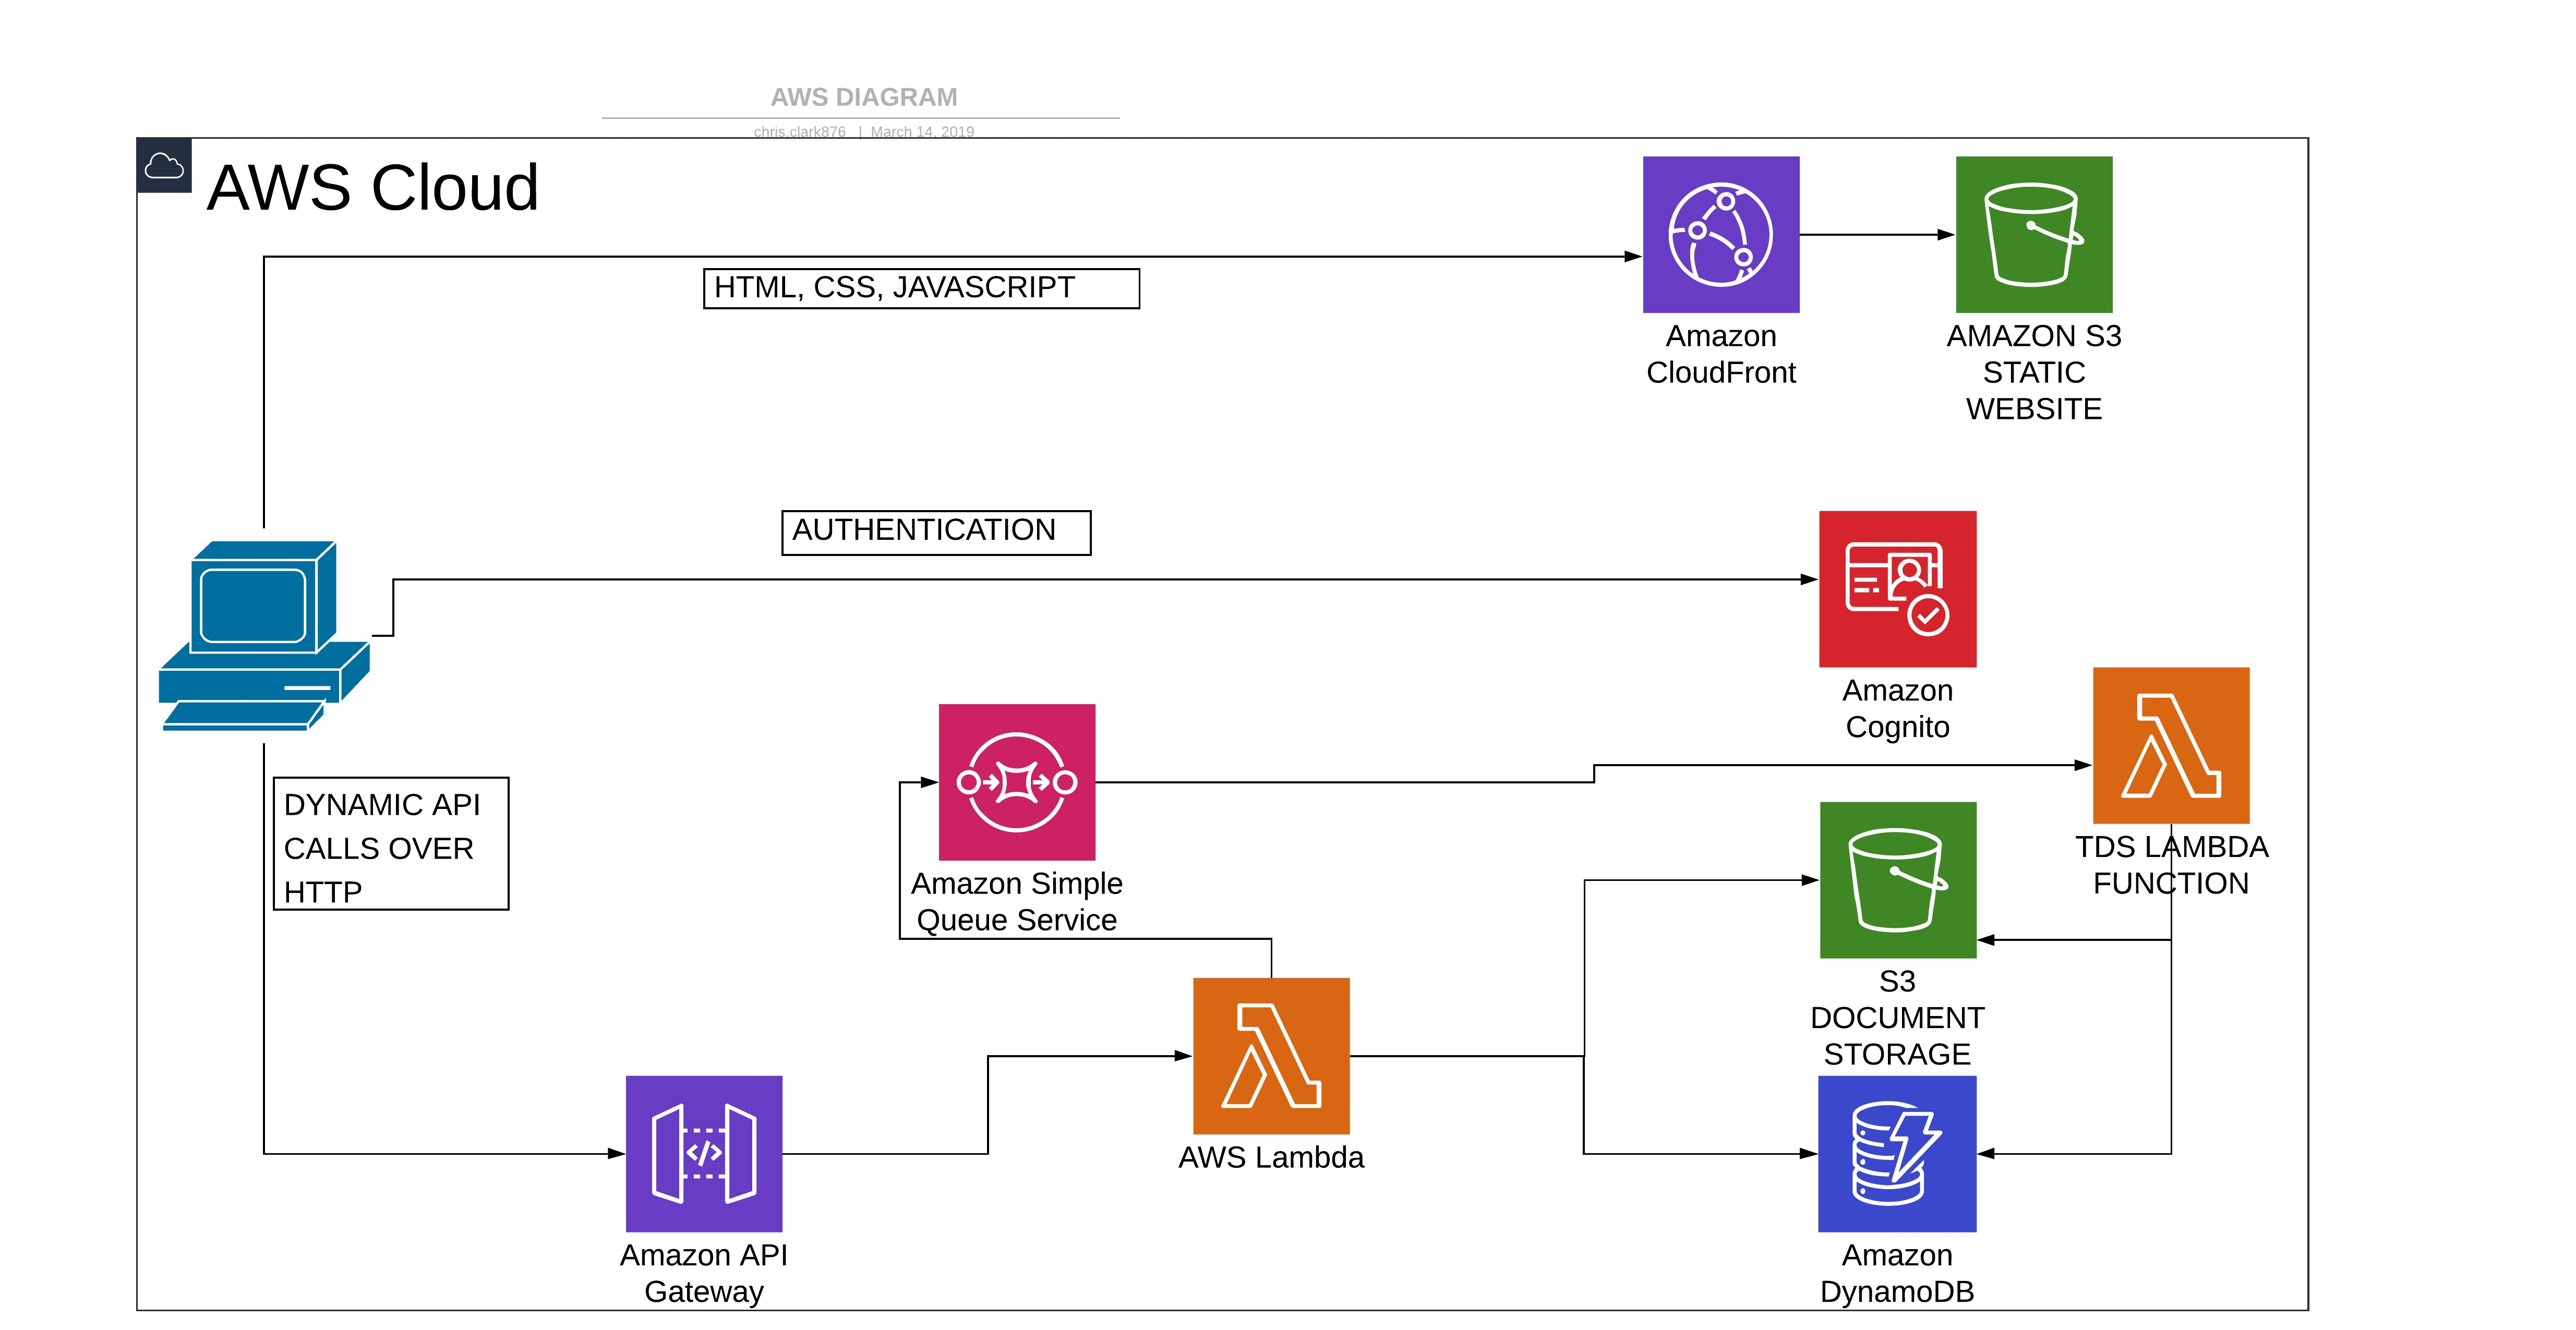
\includegraphics[width=12cm]{reportpics/11.jpg}  
		\caption{AWS Cloud}
		\label{AWS Cloud}
	\end{figure}

This diagram gives a relatively good idea of the high-level interaction of our service. This will give a high-level description of what each service is for. Later on, in the section, more detail will be given on what each service is, what is it used for, and why it was chosen over alternatives. As mentioned within the previous section. The architecture we have chosen is that of a 100\% serverless architecture. Briefly what this meant was explained in section 2, however it will become clearer as it is explained in further sections, exactly why it is being utilized.

As mentioned within the previous section. The architecture we have chosen is that of a 100\% serverless architecture. Briefly what this meant was explained in section 2, however it will become clearer as it is explained in further sections, exactly why it is being utilized. In terms of a brief description of what this diagram means.

\begin{itemize}
	\item Website's static assets (HTML/CSS/JAVASCRIPT) are being stored in an S3 bucket, as opposed to an EC2 container being served over Cloudfront
	\item Website's Authentication is being backed by an AWS service called Cognito
	\item Access to AWS services is being granted through an AWS component called API-Gateway.
	\item Backend Logic is being executed by AWS Lambda (Calling of Amazon API's, handling of creating/verifying signatures)
	\item Storage of assets (Documents/Signatures/Keys) is being handled by S3
	\item DynamoDB is used to keep track of the state of the transactions.
\end{itemize}

\subsection{Breakdown of AWS services}
As a side to the start of this section, EC2 is going to be compared against multiple components and use cases, as it has multiple. For example, it can be used to serve front end assets in the form of a web server, it can also be used to house databases/application containers.
\subsection{How is our content being served to the user?}
When I say how is our content being served to our user. This can be interpreted as what technology are we using in place of a web-server to serve our front end logic to the user.

We have opted to use S3 static website hosting served through an AWS service called Cloudfront. There are a lot of benefits to doing it this way. First of all S3 offers a multitude of benefits including:

\begin{itemize}
	\item Allows for highly available front end 99.99\%
	\item Auto load balanced
	\item Low Cost only pay for your what you use
\end{itemize}
To expand upon these bullet points. There is no server do worry about in the traditional sense here. You will only pay for the amount of times someone requests static assets from your bucket to display the website.

There is no need to worry about load balancing as this is all handled by S3.There has been one major recorded outing in the entirety of AWS's lifetime, also known as the day "the internet went down". So they can guarantee 99.99\% availability.

The reason we are using CloudFront; is that out of the box S3 static websites do not offer the protection of HTTPS and SSL. Serving our website through this method offers us these protections, as well as more control over what can be sent to our bucket; such as the controlling of allowed HTTP operations(such as only allowing GET and HEAD requests, as opposed to just post).

There are also the downsides of using something like an EC2 server to bear in mind as well when choosing how our assets are served.

If you want an EC2 instance running then you need to pay someone to apply software patches, check the disk space, make sure there is enough CPU etc, etc. Also if you go from 2 users of your platform to 1,000,000 then you will need to scale your EC2 instances which can be pain.  They will required load balancers and autoscaling groups.

This comparison can be seen as Static Website vs Dynamic Website. Static websites are gaining a lot of traction as per the above answers.  Having a dynamic website typically means database, application container (jboss / tomcat) and web server. All of the problems as pointed out in the above statements. If your content doesn't need dynamic database driven content, then it can be far cheaper to have static content served from S3.

Static S3 websites are not a bullet proof solution however, CloudFront does not offer the same amount of control as having a server hosted on EC2. So for example, if a use case required that the IP address only be accessible from Newcastle University; this isn't something CloudFront/S3 can offer you. So this may be a good use case to consider using EC2.

\subsection{How are AWS Services being accessed?}
There are multiple ways AWS services can be accessed.
\begin{enumerate}
	\item They can be accessed directly over a RESTful interface using Amazon API Gateway.
	\item They can be accessed programmatically using the AWS SDK; containedwithin a conventional code stack.
	\item Or a combination of the two can be used. Amazon API Gateway can be used to call Lambda Functions (these will be talked about in more detail further on in the section) that then perform operations upon AWSServices
\end{enumerate}
Each of these options have their merits and drawbacks.

Let's examine the first point, accessing the AWS service directly over REST. This can often be seen as a good use case, if you are wanting to call one service; and that is it. For example, if all you want to do is read something from a bucket, this makes sense. The problem with this approach relies on if your goal involves 1 or more operations relying on each other. Say for example, you want to do a database lookup, that database lookup will tell give you an S3 document location, you then want to copy that document from one bucket to another. This could be many REST requests and coordinating them can quickly become a pain.

This above drawback to just using REST calls can be solved by utilizing the AWS SDK within code. If you have a logical operation that relies on multiple AWS services working together, it is easy to call each API separately and get the overall result you need; synchronizing them is not a challenge. However, the drawback with this approach comes with having to provide your full AWS details (Secret Key etc) somewhere in the code. While there are secure ways of doing this, such as inserting them as environment variables during a DevOps process, it is an all too common occurrence for people to publish their secret keys to GitHub, and have their AWS accounts abused.

A compromise between these two solutions is using API Gateway to call Lambda functions that in turn call your AWS services. Your API call can be secured by an API  key (it can be secured further using JWT's provided by theCognito login service, but this will be discussed later in the section), no need to provide your full AWS details. And since the Lambda function is inside yourAWS account, it can securely call services from there. Lambdas can have calls to multiple calls to AWS services inside of them. The benefits and drawbacks of Lambda will be discussed later on in this section.

\subsection{How is backend logic performed?}
Backend logic is done (primarily) with code. Our backend logic consists primarily of reading and writing to a database (to keep track of our transactions); as well as reading and writing from BLOB storage(signatures, document). As well as the creation and verification of signatures. We identified two main approaches that we could take. We could either have a codebase written in a language of our choice hosted on an application server on EC2. Or we could utilize the Runtime as a Service platform known as Lambda that is offered by AWS. We have already seen the benefits of securing our AWS info by utilizing Lambda, but it has other benefits.

\subsubsection{What is Lambda?}
Lambda can be described in the following four bullet points:
\begin{itemize}
	\item Stateless functions
	\item "Single Use"
	\item Allows for Runtime as a Service
	\item Implemented in almost all languages
	\item Secures Code
\end{itemize}

It is a stateless function, which means that you SHOULD write it in a way thatit is stateless; meaning that all information that is needed to execute the function, should be contained within it, it should rely on no outside state.

Lambda functions are designed to be single use (used for only one purpose) this is a term that can be used loosely however, single use really means that the code should not be very resource intensive. If the code is doing multiple things, but it is not incurring heavy memory usage, this is fine.

It allows for the concept of Runtime as a Service. This means that you only pay for the total amount of time it takes for the code to execute. Code takes 1 second to run? You only pay for 1 second.

It is implemented in all major languages(Java, JavaScript Python, C\#, Go etc).It should be noted though, while all these languages offer the exact same API access. It is easier to work with Lambda in languages such as Python and JavaScript than it is for languages such as C\# and Java (You can't work in the Lambda GUI using these languages)

Finally, it secures code. As stated above, your AWS Credentials are automatically accessed from the Lambda function. Any sensitive information such as keys or database access credentials can be securely stored inside your Lambda code.

\subsubsection{Why Lambda?}
As mentioned above, your other option for backend logic is hosting your runtime on an application server. This means that it will be running 24/7, andif it is idle you will only pay for what you use. The benefits of using Lambda are similar to why you would use a static S3 bucket to host your content as opposed to an EC2 server. It comes with a lot of complex configuration and management when it comes to scaling your application.

If you want an EC2 instance running then you need to pay someone to apply software patches, check the disk space, make sure there is enough CPU etc, etc.  This costs money - which you don't need if you are using pure lambdas.

Also if you go from 2 users of your platform to 1,000,000 then you will need to scale your EC2 instances which can be pain.  They will required load balancers and autoscaling groups.

With Lambdas you don't have any such problems you write your code and upload it. If no one uses your service you pay 0 cents. If 1,000,000 users come along tomorrow then they are instantly scaled and you pay for what you use.

\subsubsection{Lambda isn't bulletproof}
While a lot of benefits were listed above, Lambda is far from bulletproof. There are certainly use cases where hosting your code on an EC2 instance could be the way to go. For example, if you have software that requires access to a lot of third party API's, or it cannot be guaranteed that the code will be stateless, EC2 hosted code may be the way to go. 

Finally, going back to the "single use" point, if you have an operation that is going to be very memory intensive, and it is not feasible to split it up into several Lambda functions. EC2 hosted code may again be the way to go. Lambda allows for a maximum of 3GB of memory to be utilized on every invocation.

\subsection{How Is Data Being Persisted?}
This section will look at how data is persisted in two ways. How are we keeping track of the state of each transaction (Database)? How are we storing assets such as signatures and documents (S3)?

\subsubsection{Database Selection}
There are three main choices within the AWS ecosystem to use when selecting a database.
\begin{enumerate}
	\item Amazon RDS (Relational Database Service) this has support for PostgreSQL, MariaDB, Oracle, MySQL, and Microsoft's SQL Server
	\item Amazon's DynamoDB NoSQL Database
	\item Amazon's Aurora SQL Database
\end{enumerate}

It first makes sense to compare Amazon RDS with DynamoDB and Aurora. This is because Aurora and DynamoDB have out of the box support for serverless architecture (you only pay for the amount that you use).

When using Amazon RDS there is inherent complexity with managing (not as much complexity as if you were managing it without RDS, but complexity nonetheless).

RDS has inherent complexities in provisioning and running the service. RDS is designed to be run 24/7 and, in order to run it well, will require constant monitoring (in the form of alerts) to be probing RDS to ensure it is healthy.  DynamoDB/Aurora has none of this (or rather there is, but AWS take care of that for you).  It's therefore cheaper and more reliable to run easily. RDS has it's place and if we had a bigger service we would probably need to look at it.

Also there is a cost consideration.  Running your own RDS instance 24/7 can incur large costs over the life span of the service we are running.  This isn't the case for DynamoDB/Aurora.

\subsubsection{Aurora or DynamoDB?}
Aurora and Dynamo have the following in common:

\begin{itemize}
	\item They are both serverless.
	\item Both scale very well.
	\item Both support ACID transactions.
\end{itemize}

The main draw of using something like Aurora is that it has support for PostgreSQL and MySQL. So if you have an already existing database that uses MySQL or PostgreSQL it makes a lot of sense to switch to Aurora.

The reason we have decided to use DynamoDB is that we have no pre-existing database infrastructure that we want to use, as well as it providing almost single digit response times at almost any scale.

The main use case that would mean using Aurora or DynamoDB is if you are wanting to return large amounts of data (as in millions of rows of data). If youare returning this amount of data, it makes sense to use Aurora. However, at most in this type of application we would be returning thousands (the historyof transactions for a user).

\subsubsection{BLOB Storage Selection}
In terms of BLOB storage, the main options offered by AWS are Amazon S3 and EFS. This choice was a relatively straight forward one. EFS is only offered when using an EC2 instance, which we have decided not to do. AWS S3 offers the following benefits:

\begin{itemize}
	\item Allows for highly available front end 99.99\%
	\item Encryption at Rest
	\item Low Cost only pay for your what you use
\end{itemize}

S3 has almost no down sides when it comes to using BLOB storage, and many of the benefits were listed within the using S3 as a static website.

\subsection{User Security}
There are two aspects of user security within our system. The login system and how we secure our private keys

\subsubsection{Login System}
In terms of user security, there are two approaches to take. It is possible to
\begin{itemize}
	\item Write your own login system
	\item To use an authentication API such as Passport.js,
	\item To use AWS Cognito
\end{itemize}

AWS Cognito provides out of the box basic authentication features such as MFA, email confirmation upon signing up etc.When using something like AWS Cognito it takes all the complexity out of managing sensitive items such as user passwords. The main benefit of Cognito that applies to our system is the concept of JWT's. Within our system JWT's have two uses.

\begin{itemize}
	\item Firstly, it allows us to uniquely identify our users through the use of a sub attribute. JWT's can be decoded into attributes which we see below. Within the implementation section we will see how the sub is used to uniquely and securely identify users when it comes to the TDS for storing documents and for storing keys.
	\item Secondly, within the API gateway section, it was mentioned that API keys can be used to secure access to our AWS services. When using Cognito, it allows us to use our JWT's as our API keys. This means that it is only possible to access AWS services using API gateway if the user is logged in.
\end{itemize}

\begin{figure}[H]
\centering
\subfigure[JWT]{
	\begin{minipage}[t]{0.46\linewidth}
	\centering
	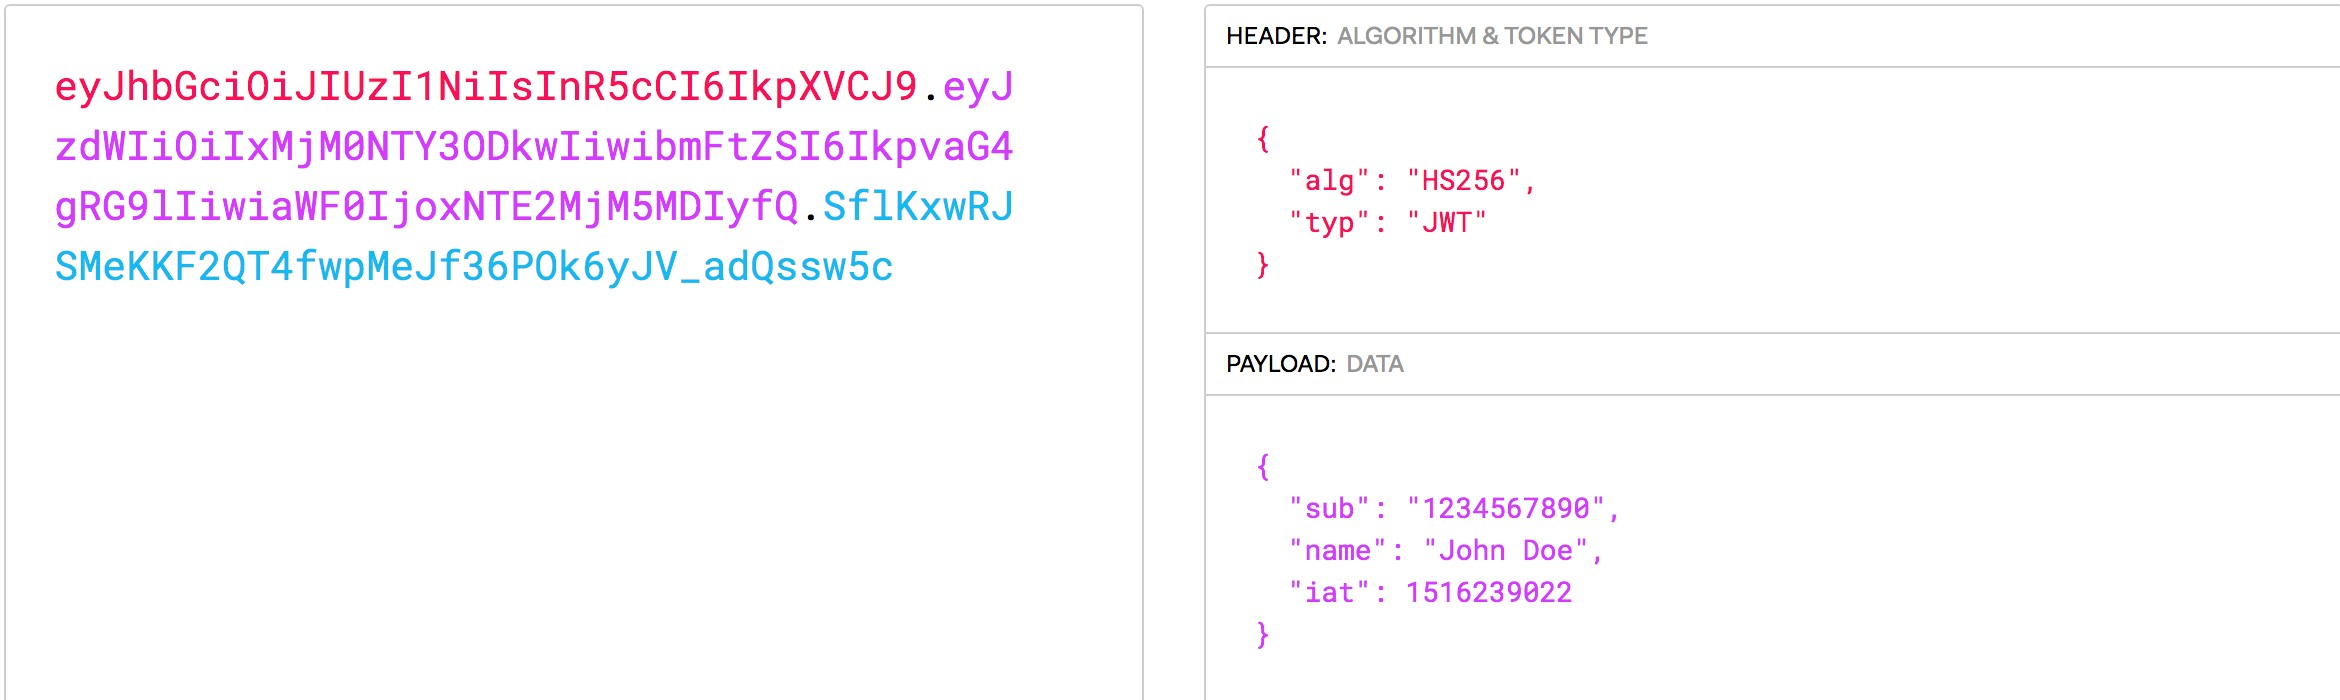
\includegraphics[width=3.0in]{reportpics/12.jpg}
	%\caption{fig1}
	\end{minipage}
}
\subfigure[S3 Folder]{
	\begin{minipage}[t]{0.46\linewidth}
	\centering
	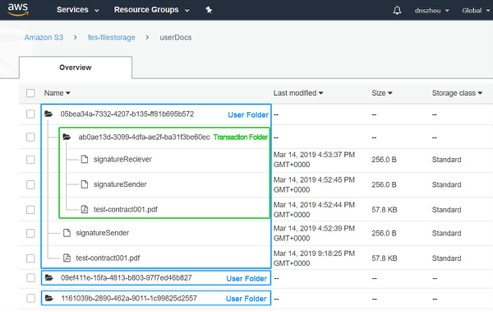
\includegraphics[width=1.6in]{reportpics/13.jpg}
	%\caption{fig1}
	\end{minipage}
}
\centering
\label{SRate}
\end{figure}

\subsubsection{Key Management}
In terms of managing keys within our system. At a high level we are storing them in S3, uniquely identified by a sub. This process will be explained in more depth within Section 5.

In terms of keys being stored within S3. They are secured from anyone outside the AWS account e.g. the users. However, it is insecure to store plaintext keys within S3, as they can be seen by the S3 bucket administrator.

In terms of keys being stored within S3. They are secured from anyone outside the AWS account e.g. the users. However, it is insecure to store plaintext keys within S3, as they can be seen by the S3 bucket administrator.

\subsubsection{Notification Services}
There are two choices when building a notification service within AWS. We can use

\begin{itemize}
	\item SQS (Simple Queue Service)
	\item SNS (Simple Notification Service)
\end{itemize}

SNS pushes messages in near real-time to all subscribers. SQS is a queueing system. Messages can't be received by multiple receiver sat the same time. Any one receiver can receive a message, process and delete it. Other receivers do not receive the same message later. SNS uses a publish subscribe architecture, which means that multiple subscribers might subscribe to a topic, when a message is sent to that topic; all subscribers will receive the message.

We have chosen to use SQS for primarily two reasons.

Our use case is that each message will only ever be sent to one person, so it doesn't make a lot of sense to use a publish-subscribe mechanism. We currently have two queues' set up. One to execute Step 2 of the protocol (Alice sends signature to Bob). Another queue to execute Step 4/5 of the protocol (Document sent to Bob, Signature sent to Alice, transaction set to resolved).

Secondly, we initially thought with the speed at which SNS can process messages, even though our architecture didn't require publish subscribe, if SNS can send ~25,000 a second, and SQS can do maximum ~3000. If it's so much faster, shouldn't we just choose SNS?

However, SQS recently introduced the ability to execute a lambda function every time a message appears in the queue. Previously, the system had to poll the queue every X seconds to process the message, thus could be possibly. With the introduction of this most recent feature, sometimes referred to as event driven architecture; this makes SQS in a lot of use cases superior to SNS.

You have observability with SQS.  If the Lambdas take 30 seconds to run, then with SNS you could only process a job once every 30 secs.  If you drop 10k jobs on SQS you can get 10k Lambdas to spin them up and the total timewill be ~30 secs.
%=============================
%=== Implementation overview and Challenges ==
%=============================
\section{Implementation overview and Challenges}

\subsection{Challenges}
During the four weeks development, we have met many challenges. Thanks to our good teamwork, we've accomplished this work perfectly. The challenges can be divide into three parts, which are cloud configuration, lambda programming and security. The details are as follows,
\begin{itemize}
	\item \textbf{Cloud Configuration}. As we use AWS serverless infrastructure, this is our first time to build a serverless system. Everything is new to us. In order to develop the application efficiency, we separate the configuration into several parts. For example, Tong take part in user system like Cognito. Because of the good communication and cooperation, we solve this problem quickly. 
	\item \textbf{Lambda Programming}. As we use Lambda function as our back-end architecture, we don't need to use Java even through Java is the only language we learned from university. Since Chris, Tong and Junyan have experience of Javascript, we chose Node.js as our backend language. It is because not only we are familiar with Javascript, but also the language consistency between front-end and back-end.
	\item \textbf{Security Issue}. Security is obviously an important work in every software development. In order to make our system as safe as possible, we apply many different strategies to protect both the user and the transactions data. For instance, we utilize HTTPs for each api to make sure all the api are security connection. And we apply private key and public key to manage our user system.
\end{itemize}


%=============================
%=== Test plan ===============
%=============================
\section{Test plan}
Testing is a very important stage in the life cycle of software development and therefore a substantial amount of time was dedicated to test this system. Table \ref{table:API Test Result} shows the result of API test, Table \ref{table:Functional Test Result} shows the result of functional test and Table \ref{table:Performance Test Result} provides the statistic data each API.

\subsection{Test strategy}
According to the testing process, this project has been strictly tested the three stages: 
\begin{itemize}
	\item \textbf{API Test}. API testing is a type of software testing that involves testing application programming interfaces (APIs) directly and as part of integration testing to determine if they meet expectations for functionality, reliability, performance, and security. We make a form for testing all APIs
	\item \textbf{Functional Test}. Functional testing is a quality assurance (QA) process\cite{wu2009qualityassurance} and a type of black-box testing that bases its test cases on the specifications of the software component under test. We also make a form for testing all functions.
	\item \textbf{Performance Test}. In software quality assurance, performance testing is a testing practice performed to determine how a system performs in terms of responsiveness, stability under a particular workload, scalability, reliability and resource usage. We utilise JMeter\cite{halili2008jemeter} as our test software which that can be used as a load testing tool for analysing and measuring the performance. We tested all APIs with multiple users and threads to make sure our system is highly accessible under high demand of transactions 
\end{itemize}

\subsection{Test result}
We conducted extensive test including api tests, functional tests and performance tests.
	\begin{table}[H] % Table
    	\centering
    	\caption{API Test Result}
    	\label{table:API Test Result} 
    	\begin{threeparttable}
    		\begin{tabular} {p{3.2cm}|p{3.8cm}|p{3.8cm}|p{1.0cm}<{\centering}}    	
    		\toprule
      		Name & Expected response &  Actual result &  Pass  \\
      		\midrule
        	uploadDocument & the location of the document & the location url of the uploaded document & Yes \\
        	\hline
        	generateEooSignature & the eoo of the document & the eoo signature of the document in BASE64 format & Yes \\
        	\hline
        	generateEorSignature & the eor of the document & the eor signature of the document in BASE64 format & Yes \\
        	\hline
        	creatTransaction & whether transaction created successfully or not & Boolean true or false & Yes \\
        	\hline
        	confirmTransaction & whether transaction created successfully or not & Boolean true or false & Yes \\
        	\hline
        	getAllUsers & all users & a list of users & Yes \\
        	\hline
        	getTransactionDetails & the imformation of the transaction & a json format data which contains the details & Yes \\
        	\hline
        	register & the location of the document & the location url of the uploaded document & Yes \\
        	\hline
        	verifySignature & the result of validation & Boolean true or false & Yes \\

      		\bottomrule
    		\end{tabular}
    		\begin{tablenotes}
          		\footnotesize
          		\item The api test result form includes the api name, the expected response, the actual result and whether the api pass the test or not. 
        	\end{tablenotes}
    	\end{threeparttable}   
	\end{table}
	
	\begin{table}[H] % Table
    	\centering
    	\caption{Functional Test Result}
    	\label{table:Functional Test Result} 
    	\begin{threeparttable}
    		\begin{tabular} {p{3.2cm}|p{3.8cm}|p{3.8cm}|p{1.0cm}<{\centering}}    	
    		\toprule
      		Name & Expected response &  Actual result &  Pass  \\
      		\midrule
        	Test upload function & file has been in S3 bucket & file has been in S3 bucket & Yes \\
        	\hline
        	Test infromation function & lastest infromation appears  & lastest infromation appears & Yes \\
        	\hline
        	Test sender's abort transaction function & both pages are aborted & Boolean true or false & Yes \\
        	\hline
        	Test EOR not match  & transaction aborted & transaction aborted & Yes \\
        	\hline
        	Test when the receiver does not receive EOO, the sender aborts & transaction aborted & transaction aborted & Yes \\
      		\bottomrule
    		\end{tabular}
    		\begin{tablenotes}
          		\footnotesize
          		\item The functional test result form includes the funtion name, the expected response, the actual result and whether the function pass the test or not. 
        	\end{tablenotes}
    	\end{threeparttable}   
	\end{table}
	
	\begin{table}[H] % Table
    	\centering
    	\caption{Performance Test Result}
    	\label{table:Performance Test Result} 
    	\begin{threeparttable}
    		\begin{tabular} {p{3.3cm}|p{2cm}<{\centering}|p{2cm}<{\centering}|p{2.5cm}<{\centering}|p{2.5cm}<{\centering}}    	
    		\toprule
      		Requsets & Response Time(ms) &  Throughput &  Network Recieved(KB/s) & Network Sent (KB/s)  \\
      		\midrule
      		Abort & 268.0 & 3.73 & 2.0 & 8.26 \\
        	\hline
        	CheckReciever & 446.0 & 2.24 & 0.71 & 5.03 \\
        	\hline
        	GetAllUsers & 2029.0 & 0.49 & 0.37 & 1.07 \\
        	\hline
        	GetInbound & 159.0 & 6.29 & 2.65 & 13.64 \\
        	\hline
        	GetOutbound & 196.0 & 5.10 & 2.15 & 11.07 \\
        	\hline
        	GetTransactionDetails & 232.0 & 4.31 & 4.36 & 9.68 \\
        	\hline
        	GetUnreadInbound & 142.0 & 7.04 & 5.32 & 15.31 \\
        	\hline
        	RetrieveURL & 100.0 & 10.00 & 11.71 & 22.21 \\
        	\hline
        	ReturnAndSaveEOR & 840.0 & 1.19 & 0.85 & 2.66 \\
        	\hline
        	Upload & 36.0 & 27.78 & 34.18 & 60.36 \\
        	\hline
        	Total & 444.8 & 2.24 & 1.65 & 4.94 \\
      		\bottomrule
    		\end{tabular}
    		\begin{tablenotes}
          		\footnotesize
          		\item This statistic form shows all APIs performance like response time, throughput and network 
        	\end{tablenotes}
    	\end{threeparttable}   
	\end{table}

%=============================
%=== Critical Evaluation =====
%=============================
\section{Critical Evaluation}
According to the development process and feedback of each group, this section will provide the insight of our system and other groups' work.
\subsection{Self-evaluation}
During our entire development, we choose serverless infrastructure after comparison of each framework. The details of serverless structure can be seen in Section 3. The serverless programming do help us a lot, the aspects of serverless design affected our project are as follows, 

\begin{itemize}
	\item \textbf{Construction Cost}. As we utilize AWS services, AWS provides a whole set of serverless services, like Lambda, S3 bucket and DynamoDB. In Lambda, we can easily invoke S3 and DynamoDB data by the specified libraries. This setting saves us a lot of developing time.
	\item \textbf{Development Efficiency}. On the other hand, we utilize node.js as our Lambda function programming language. Since we apply web browser as our system client, the front-end logic programming language which is Javascript has matched the node.js. So, it reduces our learning costs. 
	\item \textbf{Auto Scalability}. As Lambda is a FaaS(Function as a Services) which provide by AWS, it can start instance replicas as much as possible when needed without deployment and configuration delays. It depends on our stateless service.
	\item \textbf{Low Portability}. It is difficult to migrate our project to other cloud service providers, because all of our tasks was developed in AWS serverless service. If our system become a huge project, the serverless may not be a good choice.
\end{itemize}

\subsection{Relative-evaluation}
According to the infrastructure of our system, there are many different aspects between our project and other groups' project. 
\begin{itemize}
	\item \textbf{Group One}.
	\item \textbf{Group Two}.
\end{itemize}

%=============================
%=== Group working ===========
%=============================
\section{Group working}   
For any team who work together to deliver a specific product or research progress, group working is always a crucial part of the entire life cycle, especially for software development teams. Software products are so complicated that any tiny issue can crash the whole system, but software products nowadays are more and more complex that is not possible for any single developer to finish all of the work. It is especially crucial that teamwork should be standardized and constructed with specific rules.

\subsection{API Definition}
Firstly, we set a rule to define all our back-end API in a standard way with three components:
\begin{itemize}
	\item \textbf{Input:} the information that is designed to pass into the system
	\item \textbf{Process:} the internal workflow that is designed to be developed for this API
	\item \textbf{Output:} the value or information that should be returned to the outside system
\end{itemize}

\subsection{Scrum Framework}
During our project, we used the Scrum framework\cite{scrumdevelopment} as a tool to collaborate all our members and improve the efficiency of delivery.

Conventionally, develop team take some typical approach, like waterfall model, to manage their entire life-cycle of development, which means the development is following one direction from the conceptional analysis, function design, coding, testing to finally deploying and maintenance. But with the development of the software engineering industry, now more and more band new technologies are taking the place of old-style platforms of programming. More and more development team are required to keep pace with new technologies and cope with the changing requirements to follow the trend of the market. They have to find a different way to conduct their entire software production life-cycle.

Another reason for not using the waterfall model is because it takes time to understand the requirement, especially before you start to work on it\cite{sutherland2004agile}. Only after you processed to the central part of the project can you get a general idea of what you are going to make, but with waterfall model you do not have a chance to reverse the initial design and choose another path to conduct your project until you finish most of the product?

To solve these problems, we decided to take Scrum as our model during the entire developing life-cycle. Just like XP (Extreme Programming), Scrum is a kind of agile Methodology that especially suited for small develop team from3~9 members, and break the entire development work into small pieces within timeboxed iterations, which is called "Sprints." Since we only have about four weeks to develop our project, we divided the entire lifecycle into four individual Sprints. During every week we had one planning meeting on Monday, one retrospective meeting on Friday and daily stand-up meetings every day.

\begin{itemize}
	\item \textbf{Scrum Planning} is designed to discussing what we are going to deliver at the endof this sprint and decide which task we are going to finish within this sprint. Every jobshould be described clearly so that every member can understand is.
	\item \textbf{Daily Scrum} s a meeting conducted by all developing team on every workdayduring the iteration. Every group member should speak one by one, and there are onlythree topics on this meeting: what you did yesterday, what you are going to do todayand what issue or blocker during the work. This meeting is restricted to be within 15minutes, which means there is no need to describe every detail of the problem and justlet everyone else know the status of all tasks.
	\item \textbf{Sprint Retrospective} means at the end of every sprint; the team will talk and eval-uate the progress we made during this sprint, and talk about any improvements we canmake in the next sprint.
\end{itemize}

We also used Trello\cite{trelloapp} as our list-making application to help us list the status of every task undergoing, and we can easily drag them to different columns represent different status within our sprints.

	\begin{figure}[H]
		\centering
		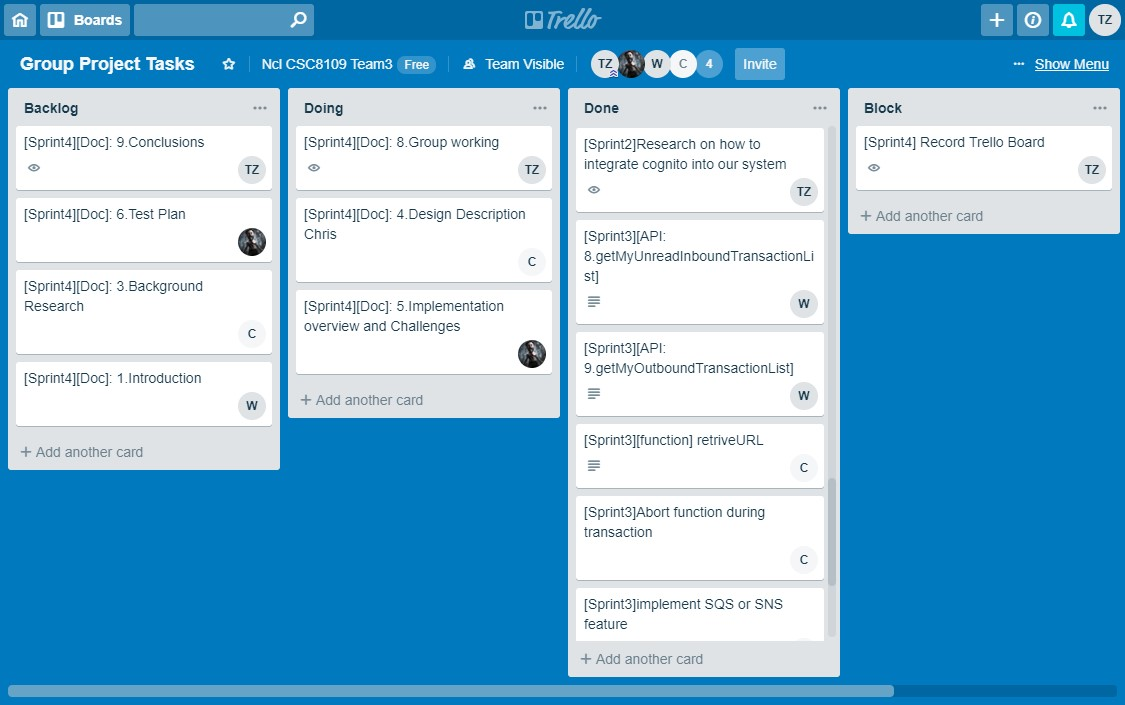
\includegraphics[width=10cm]{reportpics/10.jpg}  
		\caption{Trello Interface}
		\label{trello interface}
	\end{figure}

\subsection{Task List}
All the tasks completed during our project is listed in the table below: 
	\begin{table}[H] % Table
    	\centering
    	\caption{Contribution of each member}
    	\label{table:Contribution} 
    	\begin{threeparttable}
    		\begin{tabular} {p{7cm}|p{2.5cm}<{\centering}}
    		\toprule
      		Task & Owner  \\
      		\midrule
        	(Sprint1) Design front-end webpage for creating new exchange transaction & Tong\\
        	\hline
        	(Sprint1) Research on encryption library with Node JS & Christopher\\
        	\hline
        	(Sprint1) Research on how to do CRD with Lambda, DynamoDB anduse Postman to test it & Weicheng\\
        	\hline
        	(Sprint1) Research on upload process using lambda and S3 bucket & Weicheng\\
        	\hline
        	(Sprint1) API: 1.uploadDocument & Junyan\\
        	\hline
        	(Sprint1) API: 6.getAllUsers & Tong\\
        	\hline
        	(Sprint1) API: Login with Cognito system & Tong\\
        	\hline
        	(Sprint2) API: 10.getTransactionDetails & Tong\\
        	\hline
        	(Sprint2) API: 11.register & Tong\\
        	\hline
        	(Sprint2) API: 12.verifySignature & Christopher\\
        	\hline
        	(Sprint2) API: 2.generateEooSignature & Christopher\\
        	\hline
        	(Sprint2) API: 3.generateEorSignature & Christopher\\
        	\hline
        	(Sprint2) API: 4.creatTransaction & Junyan\\
        	\hline
        	(Sprint2) API: 5.confirmTransaction & Junyan\\
        	\hline
        	(Sprint2) Design confirm Transaction web page & Tong\\
        	\hline
        	(Sprint2) Design the APIs to be created in our system & Tong\\
        	\hline
        	(Sprint2) Generate a private key and public key(within API 11.register) & Christopher\\
        	\hline
        	(Sprint2) Research on how to integrate Cognito into our system & Tong\\
        	\hline
        	(Sprint3) API: 8.getMyUnreadInboundTransactionList & Weicheng\\
        	\hline
        	(Sprint3) API: 9.getMyOutboundTransactionList & Weicheng\\
        	\hline
        	(Sprint3) RetriveURL & Christopher\\
        	\hline
        	(Sprint3) Abort function during the transaction & Christopher\\
        	\hline
        	(Sprint3) Implement SQS or SNS feature & Christopher\\
        	\hline
 
      		\bottomrule
    		\end{tabular}
    	\end{threeparttable}   
	\end{table}


And Table \ref{table:Contribution} is a general conclusion of the contribution of each group member:
	\begin{table}[H] % Table
    	\centering
    	\caption{Contribution of each member}
    	\label{table:Contribution} 
    	\begin{threeparttable}
    		\begin{tabular} {p{2.5cm}|p{7cm}|p{2.5cm}<{\centering}}
    		\toprule
      		Name & Contribution & Total percentage \\
      		\midrule
        	Tong Zhou180275186 & Workflow   design,   teamwork   assigningand front-end and back-end programming. & 25\% \\
        	\hline
        	Junyan Wang170127567 & Back-end and front-end programming, S3,and API operations. & 25\% \\
        	\hline
        	Weicheng Yang170152145 & Front-end   and   Back-end   programming,Functional and performance test. & 25\% \\
        	\hline
        	Christopher Clark180614318 & Cloud   architecture,   back-end   program-ming, and encryption algorithms & 25\% \\
 
      		\bottomrule
    		\end{tabular}
    	\end{threeparttable}   
	\end{table}


\section{Conclusion}

\newpage
\bibliographystyle{plain}
\bibliography{reference}

\newpage
\section{Appendix}

\end{document}